z\documentclass[11pt,a4paper]{article}
\usepackage[utf8]{inputenc}
\usepackage[spanish]{babel}
\usepackage{geometry}
\geometry{left=2.5cm,right=2.5cm,top=2.5cm,bottom=2.5cm}
\usepackage{booktabs}
\usepackage{amsmath}
\usepackage{tabularx}
\usepackage{graphicx} % Paquete fundamental para insertar las graficas
\usepackage{float}    % Para forzar la posicion de las imagenes
\usepackage{hyperref}
\usepackage{listings}



% ==========================================
% PAQUETES PARA CÓDIGO FUENTE (HPC)
% ==========================================
\usepackage{listings}
\usepackage{xcolor}

\definecolor{codegreen}{rgb}{0,0.6,0}
\definecolor{codegray}{rgb}{0.5,0.5,0.5}
\definecolor{codepurple}{rgb}{0.58,0,0.82}
\definecolor{backcolour}{rgb}{0.95,0.95,0.92}

\lstdefinestyle{estiloC}{
    backgroundcolor=\color{backcolour},   
    commentstyle=\color{codegreen},
    keywordstyle=\color{magenta},
    numberstyle=\tiny\color{codegray},
    stringstyle=\color{codepurple},
    basicstyle=\ttfamily\footnotesize,
    breakatwhitespace=false,         
    breaklines=true,                 
    captionpos=b,                    
    keepspaces=true,                 
    numbers=left,                    
    numbersep=5pt,                  
    showspaces=false,                
    showstringspaces=false,
    showtabs=false,                  
    tabsize=2
}

\lstset{style=estiloC}

\title{\textbf{Proyecto de Computación de Alto Rendimiento (HPC): \\ Paralelización de la Ecuación de Poisson en 2D con OpenMP}}
\author{
    \begin{tabular}{c}
    Camilo Huertas \quad Sebastián Rodriguez \\
    \textit{Programa Académico de Física} \\
    \textit{Universidad Distrital Francisco José de Caldas} \\
    \end{tabular}
}
\date{24 de marzo de 2026}

\begin{document}

\maketitle

\section*{Objetivo}
Aplicar diferentes directivas de OpenMP para paralelizar un código secuencial que resuelve la ecuación de Poisson 2D mediante diferencias finitas. Se realizará un barrido paramétrico masivo variando la densidad de la grilla espacial y el número de hilos de procesamiento para evaluar la escalabilidad, los cuellos de botella de memoria y el límite de aceleración (Ley de Amdahl).

\section*{Especificaciones del Sistema y Metodología}
Todas las pruebas de rendimiento registradas en este informe fueron ejecutadas en un servidor HPC con la siguiente configuración:
\begin{itemize}
    \item \textbf{Procesador:} AMD Ryzen Threadripper 3990X 64-Core Processor.
    \item \textbf{Arquitectura:} x86\_64.
    \item \textbf{Caché L3:} 256 MiB.
    \item \textbf{Núcleos físicos:} 64.
    \item \textbf{Hilos lógicos (\textit{Threads}):} 128.
\end{itemize}

\textit{Nota metodológica:} En lugar de realizar una prueba estática, se programó un entorno de automatización (Makefile + script en C++) para realizar un barrido variando las mallas espaciales ($M \times N$) en tamaños de $64\times64$, $128\times128$ , $256\times256$, $512\times512$ y $1024\times1024$. Para cada escenario se forzó explícitamente el uso de  4, 8, 16, 32, y 64 hilos físicps  mediante \texttt{omp\_set\_num\_threads()}.

\section*{Análisis de Escalabilidad Visual}

En la siguiente figura se exponen las curvas de rendimiento computacional para los cinco tamaños de malla estudiados ($64, 128, 256, 512$ y $1024$). Se observa una escala logarítmica tanto en el número de hilos (eje X) como en el tiempo de ejecución (eje Y).

\begin{figure}[H]
    \centering
    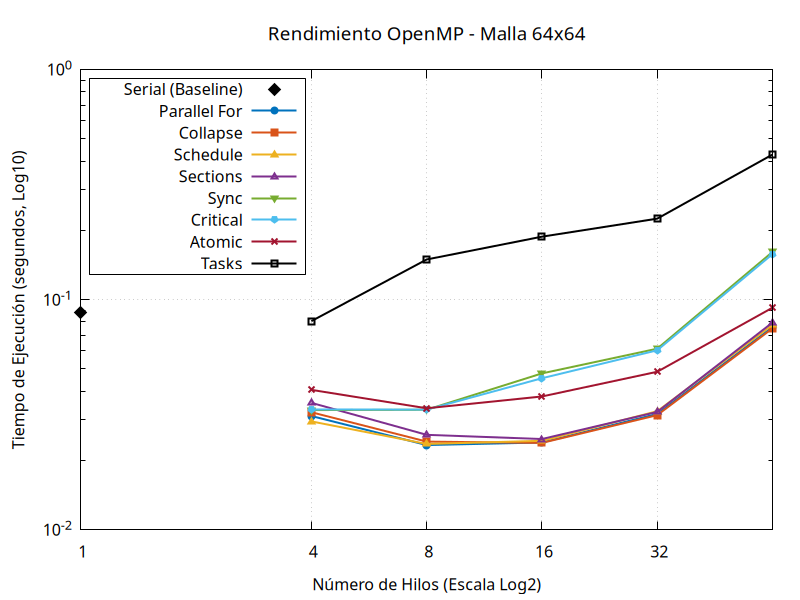
\includegraphics[width=0.45\textwidth]{../../imag/comparativa_malla_64.png}
    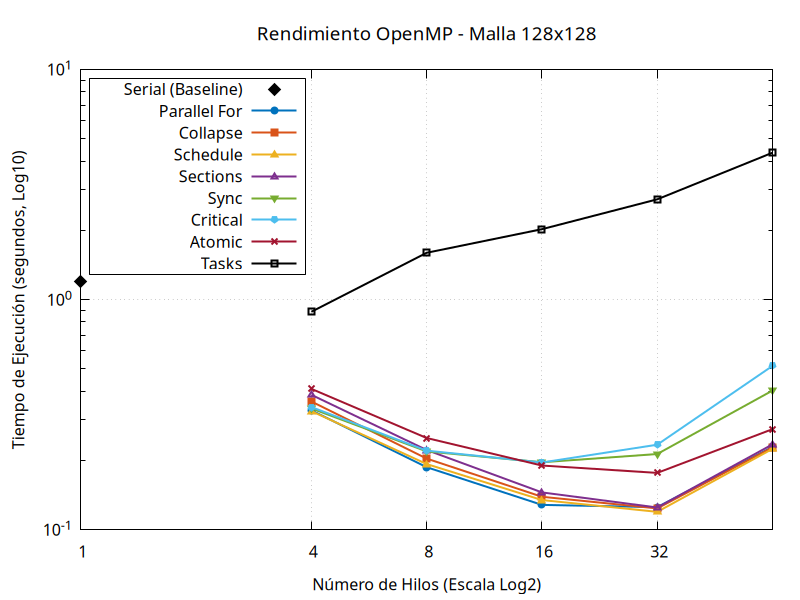
\includegraphics[width=0.45\textwidth]{../../imag/comparativa_malla_128.png} \\
    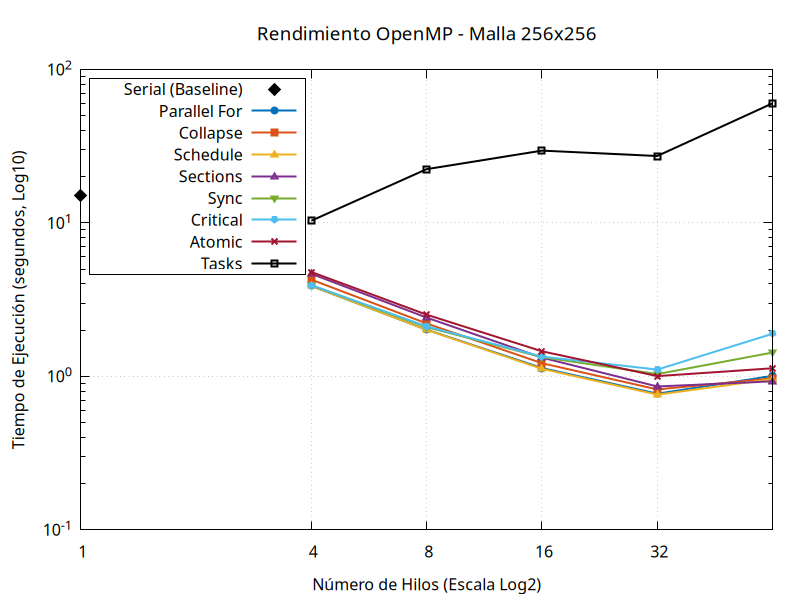
\includegraphics[width=0.45\textwidth]{../../imag/comparativa_malla_256.png}
    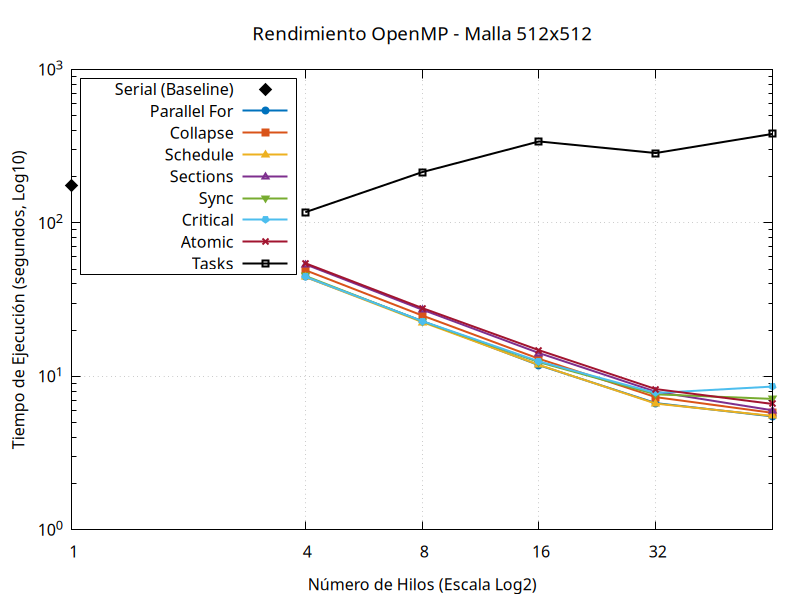
\includegraphics[width=0.45\textwidth]{../../imag/comparativa_malla_512.png} \\
    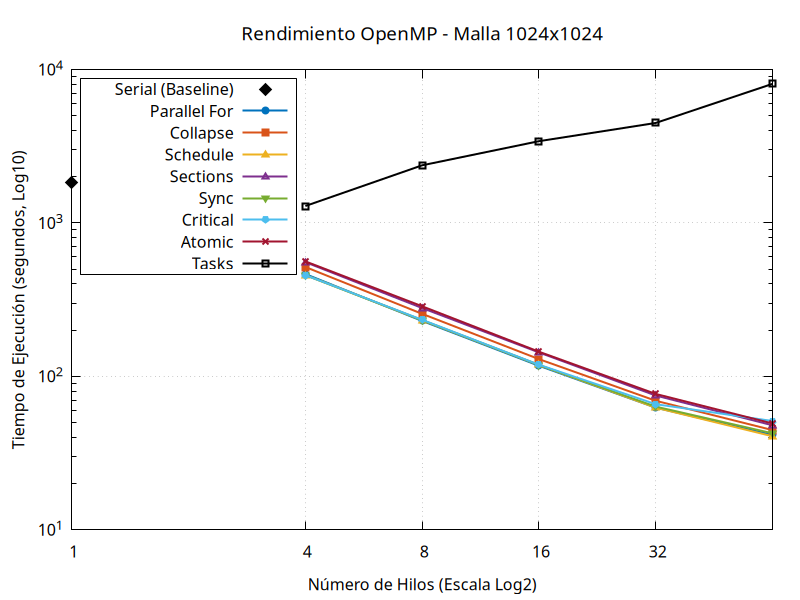
\includegraphics[width=0.7\textwidth]{../../imag/comparativa_malla_1024.png}
    \caption{Curvas de rendimiento para mallas desde 64x64 hasta 1024x1024.}
    \label{fig:rendimiento_completo}
\end{figure}

Como se evidencía en las grafícas se puede observar que dependiendo del tamaño de la malla se encuentra un pico de eficiencia para cada problema por separado en un numero de hilos diferente, a diferencia de que tanto en las mallas de 128 y las de 256 el pico se encuentra en \textbf{32 hilos}, de 512 en adelante se evidencía que las pruebas hechas con los \textbf{65 hilos} son las que llevan la ventaja. 

\section*{Análisis por Directivas}

A contincación se presentaran los resultados de las las diferentes implementacíones hechas al codigo base con el fin de entender el impacto de cada una de ellas, y ver como ganan o pierden relevancia a medida que cambiamos la magnitud del problema. 

\subsection*{Preparación}

\begin{table}[H]
\centering
\renewcommand{\arraystretch}{1.2}
\begin{tabular}{|c|c|c|c|l|}
\hline
\textbf{Tamaño de Malla ($N$)} & \textbf{Hilos} & \textbf{Tiempo de ejecución (s)} & \textbf{Iteraciones} & \textbf{Programa} \\ \hline
64 & 1 & 0.0876937 & 3136 & serial \\ \hline
128 & 1 & 1.19409 & 10244 & serial \\ \hline
256 & 1 & 15.1318 & 31844 & serial \\ \hline
512 & 1 & 176.55 & 91868 & serial \\ \hline
1024 & 1 & 1822.81 & 236161 & serial \\ \hline
\end{tabular}
\caption{Resultados de ejecución y convergencia para el código base secuencial variando el tamaño de la malla con una tolerancia de $Tol=1 \times 10 ^ {-6} $.}
\label{tab:resultados_secuenciales}
\end{table}


\subsection*{Actividad 1: Paralelización con \texttt{\#pragma omp parallel for}}

\subsubsection*{1. Implementación y Mecánica}
En esta fase se implementó la paralelización del bucle de mayor granularidad dentro de la subrutina \texttt{solve\_poisson}. La estrategia consistió en distribuir las iteraciones del bucle espacial externo (índice $i$) entre los hilos disponibles en el bloque \texttt{parallel}, garantizando la integridad de la variable de convergencia mediante una reducción de norma infinito ($L_\infty$). 

La directiva fue implementada en el archivo \texttt{poisson\_parallel\_for.cpp} de la siguiente manera:

\begin{lstlisting}[language=C++, caption={Fragmento de paralelización del bucle principal en \texttt{solve\_poisson}.}, label={lst:act1}]
void solve_poisson(std::vector<std::vector<double>>& T, const std::vector<std::vector<double>>& source, int M, int N, double h, double k, double TOL_param) {
    double delta = 1.0;
    
    while (delta > TOL_param) {
        delta = 0.0;
        
        // Sincronización optimizada mediante reducción atómica de OpenMP
        #pragma omp parallel for reduction(max:delta)
        for (int i = 1; i < M; ++i){
            for (int j = 1; j < N; ++j){
                double T_old = T[i][j];
                
                // Discretización por diferencias finitas (esquema centrado)
                T[i][j] = (((T[i+1][j] + T[i-1][j]) * k*k) + ((T[i][j+1] + T[i][j-1]) * h*h) - (source[i][j] * h*h*k*k)) / (2.0 * (h*h + k*k));
                
                // Cálculo del residuo local
                double diff = std::abs(T[i][j] - T_old);
                if (diff > delta) {
                    delta = diff;
                }
            }
        }
        iterations++;
    }
}
\end{lstlisting}

\subsubsection*{2. Resultados de Escalabilidad}

A continuación, se presentan los tiempos de ejecución (en segundos) para la directiva \texttt{parallel\_for} en todas las configuraciones de malla evaluadas.

\begin{table}[H]
\centering
\renewcommand{\arraystretch}{1.2}
\small
\begin{tabular}{|c|c|c|c|c|}
\hline
\textbf{Malla ($N$)} & \textbf{Hilos ($p$)} & \textbf{Tiempo (s)} & \textbf{Iteraciones} & \textbf{Speedup $S(p)$} \\ \hline
64 & 1 (Serial) & 0.0876937 & 3136 & 1.00x \\ 
64 & 4 & 0.0312039 & 3134 & 2.81x \\ 
64 & 8 & 0.0233430 & 3133 & 3.76x \\ 
64 & 16 & 0.0239537 & 3129 & 3.66x \\ 
64 & 32 & 0.0318738 & 3188 & 2.75x \\ 
64 & 64 & 0.0760424 & 4336 & 1.15x \\ \hline
128 & 1 (Serial) & 1.1940900 & 10244 & 1.00x \\ 
128 & 4 & 0.3302590 & 10242 & 3.61x \\ 
128 & 8 & 0.1870150 & 10241 & 6.38x \\ 
128 & 16 & 0.1282790 & 10237 & 9.31x \\ 
128 & 32 & 0.1254010 & 10230 & 9.52x \\ 
128 & 64 & 0.2291600 & 10601 & 5.21x \\ \hline
256 & 1 (Serial) & 15.131800 & 31844 & 1.00x \\ 
256 & 4 & 3.8845700 & 31842 & 3.89x \\ 
256 & 8 & 2.0132600 & 31840 & 7.51x \\ 
256 & 16 & 1.1325100 & 31837 & 13.36x \\ 
256 & 32 & 0.7708850 & 31830 & 19.63x \\ 
256 & 64 & 1.0072800 & 31817 & 15.02x \\ \hline
512 & 1 (Serial) & 176.55000 & 91868 & 1.00x \\ 
512 & 4 & 44.499800 & 91867 & 3.97x \\ 
512 & 8 & 22.923300 & 91865 & 7.70x \\ 
512 & 16 & 11.820200 & 91862 & 14.93x \\ 
512 & 32 & 6.6926400 & 91855 & 26.38x \\ 
512 & 64 & 5.4785900 & 91842 & 32.22x \\ \hline
1024 & 1 (Serial) & 1822.8100 & 236161 & 1.00x \\ 
1024 & 4 & 464.33700 & 236161 & 3.93x \\ 
1024 & 8 & 229.70800 & 236159 & 7.94x \\ 
1024 & 16 & 117.20200 & 236156 & 15.55x \\ 
1024 & 32 & 62.507700 & 236150 & 29.16x \\ 
1024 & 64 & 41.494000 & 236138 & 43.93x \\ \hline
\end{tabular}
\caption{Desempeño de \texttt{parallel\_for} para distintos tamaños de malla y conteo de hilos.}
\label{tab:resultados_parallel_for}
\end{table}
\subsubsection*{3. Análisis Técnico y Respuestas}

\begin{enumerate}
    \item \textbf{¿Por qué es necesaria la cláusula \texttt{reduction}?} \\
    Es imperativa para evitar \textit{data races}. La variable \texttt{delta} acumula el error máximo de la malla. Sin \texttt{reduction(max:delta)}, múltiples hilos intentarían sobreescribir esta variable compartida simultáneamente. Esta cláusula permite que cada hilo calcule un máximo local privado, combinándolos de forma atómica y segura al finalizar la región paralela.

    \item \textbf{¿Hubo mejora de rendimiento?} \\
    Sí, logrando un escalamiento fuerte (\textit{Strong Scaling}) evidente en mallas grandes (ej. \textit{Speedup} de \textbf{43.93x} en $1024 \times 1024$ con 64 hilos). Sin embargo, en mallas pequeñas ($64 \times 64$), usar más de 8 hilos degrada el rendimiento. Esto ilustra la Ley de Amdahl: el \textit{overhead} del sistema operativo para gestionar los hilos supera el beneficio computacional al tener una carga de trabajo tan reducida.

    \item \textbf{¿Hubo diferencia en el número de iteraciones?} \\
    Sí, existe una ligera variación. Al actualizar la matriz \textit{in-place} mediante múltiples hilos, se rompe el orden estricto secuencial (Gauss-Seidel puro). Las lecturas y escrituras concurrentes generan un comportamiento no determinista en la propagación del error, alterando sutilmente la iteración exacta en la que el residuo global cumple la tolerancia.
\end{enumerate}

\subsubsection*{4. Veredicto Arquitectónico}
\textbf{¿Valió la pena?} Absolutamente. Es la directiva con la mejor relación costo-beneficio del laboratorio debido a su mínima necesidad de refactorización. \textbf{¿Cuándo usarla?} En bucles intensivos donde las iteraciones sean estrictamente independientes. No obstante, en la resolución de EDPs, para garantizar un determinismo numérico del 100\%, debe combinarse con esquemas algorítmicos paralelos seguros, como el método de Jacobi o el coloreo \textit{Red-Black}.



\subsection*{Actividad 2: Aceleración con anidamiento de bucles (\texttt{collapse})}

\subsubsection*{1. Implementación y Mecánica}
Se modificó la subrutina \texttt{solve\_poisson} para fusionar los dos bucles espaciales ($i$ y $j$) en un único espacio de iteración lineal de tamaño $(M-1) \times (N-1)$. Esto incrementa la cantidad total de tareas independientes que el planificador de OpenMP puede distribuir entre los hilos.

\begin{lstlisting}[language=C++, caption={Implementación de collapse en \texttt{poisson\_collapse.cpp}}, label={lst:act2}]
// El collapse(2) fusiona los bucles de i y j en un solo bloque lineal
#pragma omp parallel for collapse(2) reduction(max:delta)
for (int i = 1; i < M; ++i) {
    for (int j = 1; j < N; ++j) {
        // Discretización y cálculo del residuo
\end{lstlisting}

\subsubsection*{2. Resultados de Escalabilidad}
Los tiempos de ejecución (en segundos) para la variante con \texttt{collapse(2)} se detallan a continuación.

\begin{table}[H]
\centering
\renewcommand{\arraystretch}{1.2}
\small
\begin{tabular}{|c|c|c|c|c|}
\hline
\textbf{Malla ($N$)} & \textbf{Hilos ($p$)} & \textbf{Tiempo (s)} & \textbf{Iteraciones} & \textbf{Speedup $S(p)$} \\ \hline
64 & 1 (Serial) & 0.0876937 & 3136 & 1.00x \\ 
64 & 4 & 0.0324098 & 3134 & 2.71x \\ 
64 & 8 & 0.0241590 & 3133 & 3.63x \\ 
64 & 16 & 0.0238478 & 3129 & 3.68x \\ 
64 & 32 & 0.0314899 & 3137 & 2.78x \\ 
64 & 64 & 0.0750466 & 4125 & 1.17x \\ \hline
128 & 1 (Serial) & 1.1940900 & 10244 & 1.00x \\ 
128 & 4 & 0.3608980 & 10242 & 3.31x \\ 
128 & 8 & 0.2038680 & 10241 & 5.86x \\ 
128 & 16 & 0.1391100 & 10237 & 8.58x \\ 
128 & 32 & 0.1238410 & 10230 & 9.64x \\ 
128 & 64 & 0.2280480 & 10536 & 5.24x \\ \hline
256 & 1 (Serial) & 15.131800 & 31844 & 1.00x \\ 
256 & 4 & 4.2694700 & 31842 & 3.54x \\ 
256 & 8 & 2.2104100 & 31840 & 6.85x \\ 
256 & 16 & 1.2177500 & 31837 & 12.43x \\ 
256 & 32 & 0.8218210 & 31830 & 18.41x \\ 
256 & 64 & 0.9711080 & 31817 & 15.58x \\ \hline
512 & 1 (Serial) & 176.55000 & 91868 & 1.00x \\ 
512 & 4 & 49.186000 & 91867 & 3.59x \\ 
512 & 8 & 24.932800 & 91865 & 7.08x \\ 
512 & 16 & 13.019500 & 91862 & 13.56x \\ 
512 & 32 & 7.3178200 & 91855 & 24.13x \\ 
512 & 64 & 5.7811900 & 91842 & 30.54x \\ \hline
1024 & 1 (Serial) & 1822.8100 & 236161 & 1.00x \\ 
1024 & 4 & 516.07000 & 236161 & 3.53x \\ 
1024 & 8 & 255.44800 & 236159 & 7.14x \\ 
1024 & 16 & 129.47600 & 236156 & 14.08x \\ 
1024 & 32 & 69.310000 & 236150 & 26.30x \\ 
1024 & 64 & 44.623200 & 236139 & 40.85x \\ \hline
\end{tabular}
\caption{Desempeño de \texttt{collapse(2)} para distintos tamaños de malla y conteo de hilos.}
\label{tab:resultados_collapse}
\end{table}
\subsubsection*{3. Análisis Técnico y Respuestas}

\begin{enumerate}
    \item \textbf{¿Qué hace \texttt{collapse(2)}?} \\
    Toma dos bucles anidados perfectamente estructurados y los trata algorítmicamente como un único bucle de tamaño $I \times J$. Esto amplía el espacio de iteraciones disponible, dándole al \textit{scheduler} de OpenMP más granularidad para distribuir el trabajo entre los hilos de manera equitativa.

    \item \textbf{¿Mejoró respecto a la versión anterior (\texttt{parallel for})?} \\
    \textbf{No.} Al observar los datos, \texttt{collapse(2)} es consistentemente más lento que un simple \texttt{parallel for}. Por ejemplo, en $512 \times 512$ con 64 hilos, \texttt{collapse} tarda $5.82s$, mientras que la versión base tardaba $5.49s$. 

    \item \textbf{¿Es siempre recomendable su uso?} \\
    No. En mallas cuadradas continuas en memoria (como una matriz en C++ anidando \texttt{std::vector}), el bucle externo suele proporcionar suficiente paralelismo si $M \gg p$ (tamaño de la malla mucho mayor que el número de hilos). Forzar el \texttt{collapse} en este escenario solo introduce \textit{overhead} adicional por el cálculo de índices lineales internos sin ofrecer un beneficio de balanceo de carga real.
\end{enumerate}

\subsubsection*{4. Veredicto Arquitectónico}
Para este problema en específico, \texttt{collapse} resulta subóptimo. Su uso está justificado únicamente cuando el bucle más externo es muy pequeño (ej. iterar sobre 4 elementos) y no hay suficiente trabajo para alimentar a todos los hilos, obligando a extraer paralelismo de los bucles internos.


\subsection*{Actividad 3: Paralelismo de tareas independientes (\texttt{sections})}

\subsubsection*{1. Implementación y Mecánica}
Se utilizó la directiva \texttt{\#pragma omp sections} para ejecutar la inicialización de las fronteras espaciales y la matriz fuente de forma concurrente. Cada función fue delegada a un hilo distinto mediante \texttt{\#pragma omp section}.

\begin{lstlisting}[language=C++, caption={Implementación de sections en el programa principal.}, label={lst:act3}]
// Asignación de memoria obligatoria en el hilo maestro (serial)
std::vector<std::vector<double>> T(M+1, std::vector<double>(N+1, 0.0));
std::vector<std::vector<double>> source(M+1, std::vector<double>(N+1, 0.0));

// Bifurcación de tareas independientes
#pragma omp parallel sections
{
    #pragma omp section
    initialize_boundaries(M, N, T, h, k); // Ejecutado por Hilo 0

    #pragma omp section
    poisson_source(M, N, source);         // Ejecutado por Hilo 1
}
\end{lstlisting}

\subsubsection*{2. Resultados de Escalabilidad}
A continuación se muestran los tiempos totales de ejecución integrando la inicialización por secciones y la resolución de Poisson.

\begin{table}[H]
\centering
\renewcommand{\arraystretch}{1.2}
\small
\begin{tabular}{|c|c|c|c|c|}
\hline
\textbf{Malla ($N$)} & \textbf{Hilos ($p$)} & \textbf{Tiempo (s)} & \textbf{Iteraciones} & \textbf{Speedup $S(p)$} \\ \hline
64 & 1 (Serial) & 0.0876937 & 3136 & 1.00x \\ 
64 & 4 & 0.0356070 & 3135 & 2.46x \\ 
64 & 8 & 0.0258548 & 3133 & 3.39x \\ 
64 & 16 & 0.0247927 & 3129 & 3.54x \\ 
64 & 32 & 0.0325148 & 3167 & 2.70x \\ 
64 & 64 & 0.0795554 & 4127 & 1.10x \\ \hline
128 & 1 (Serial) & 1.1940900 & 10244 & 1.00x \\ 
128 & 4 & 0.3857880 & 10242 & 3.10x \\ 
128 & 8 & 0.2221100 & 10241 & 5.38x \\ 
128 & 16 & 0.1453310 & 10237 & 8.22x \\ 
128 & 32 & 0.1249500 & 10230 & 9.56x \\ 
128 & 64 & 0.2350350 & 10864 & 5.08x \\ \hline
256 & 1 (Serial) & 15.131800 & 31844 & 1.00x \\ 
256 & 4 & 4.6567700 & 31842 & 3.25x \\ 
256 & 8 & 2.4143200 & 31840 & 6.27x \\ 
256 & 16 & 1.3243100 & 31837 & 11.43x \\ 
256 & 32 & 0.8590700 & 31830 & 17.61x \\ 
256 & 64 & 0.9283690 & 31817 & 16.30x \\ \hline
512 & 1 (Serial) & 176.55000 & 91868 & 1.00x \\ 
512 & 4 & 53.706000 & 91867 & 3.29x \\ 
512 & 8 & 27.230100 & 91865 & 6.48x \\ 
512 & 16 & 14.185700 & 91862 & 12.45x \\ 
512 & 32 & 7.9406200 & 91855 & 22.23x \\ 
512 & 64 & 6.0056200 & 91843 & 29.40x \\ \hline
1024 & 1 (Serial) & 1822.8100 & 236161 & 1.00x \\ 
1024 & 4 & 555.12700 & 236161 & 3.28x \\ 
1024 & 8 & 278.73400 & 236159 & 6.54x \\ 
1024 & 16 & 143.21200 & 236156 & 12.73x \\ 
1024 & 32 & 74.973000 & 236150 & 24.31x \\ 
1024 & 64 & 47.961900 & 236138 & 38.00x \\ \hline
\end{tabular}
\caption{Desempeño general utilizando \texttt{sections} en la inicialización.}
\label{tab:resultados_sections}
\end{table}
\subsubsection*{3. Análisis Técnico y Respuestas}

\begin{enumerate}
    \item \textbf{¿Tuviste que reordenar las funciones? ¿Por qué?} \\
    Sí, fue estrictamente necesario. En la versión secuencial, \texttt{initialize\_grid} asignaba la memoria dinámica. Al usar \texttt{sections}, asignar memoria en un hilo mientras otro intenta escribir en ella genera una condición de carrera sobre el gestor de memoria (\textit{Heap}) o un \textit{Segmentation Fault}. La memoria debió reservarse previamente en el hilo maestro antes de la región paralela.

    \item \textbf{¿Vale la pena paralelizar funciones tan rápidas?} \\
    \textbf{No.} La inicialización tiene una complejidad $O(N^2)$ muy baja comparada con la resolución de Poisson que ejecuta miles de iteraciones. El \textit{overhead} temporal impuesto por el sistema operativo para crear la región paralela, despachar los hilos y sincronizarlos supera con creces el cálculo aritmético en sí mismo.
\end{enumerate}

\subsubsection*{4. Veredicto Arquitectónico}
Para inicializar datos o realizar bucles triviales, \texttt{sections} es contraproducente debido a la fuerte penalización por sincronización. Esta directiva está diseñada para paralelismo de grano grueso (\textit{Task-level parallelism}), como operaciones asimétricas (ej. un hilo realiza I/O en disco mientras otro procesa datos en memoria), y no para micro-optimizaciones matriciales.
\subsection*{Actividad 4: Control explícito de la región paralela y \texttt{schedule}}

\subsubsection*{1. Implementación y Mecánica}
Se separó la creación de los hilos de la distribución del trabajo. Al abrir una región \texttt{\#pragma omp parallel}, los hilos se instancian una sola vez. Dentro de ella, el \texttt{\#pragma omp for} reparte el bucle espacial iterativo. Se impuso explícitamente un \texttt{schedule(static)}, el cual divide el espacio de iteraciones en bloques continuos de igual tamaño asignados a cada hilo en tiempo de compilación.

\begin{lstlisting}[language=C++, caption={Separación de la región paralela y particionamiento estático.}, label={lst:act4}]
// 1. Creación del equipo de hilos (Fork)
#pragma omp parallel
{
    // 2. Distribución de carga de trabajo precalculada
    #pragma omp for schedule(static) reduction(max:delta)
    for (int i = 1; i < M; ++i) {
        for (int j = 1; j < N; ++j) {
            // Discretización de Poisson (Carga FLOP uniforme)
\end{lstlisting}

\subsubsection*{2. Resultados de Escalabilidad}
Los tiempos y factores de aceleración para la variante con \texttt{schedule(static)} se reportan a continuación.

\begin{table}[H]
\centering
\renewcommand{\arraystretch}{1.2}
\small
\begin{tabular}{|c|c|c|c|c|}
\hline
\textbf{Malla ($N$)} & \textbf{Hilos ($p$)} & \textbf{Tiempo (s)} & \textbf{Iteraciones} & \textbf{Speedup $S(p)$} \\ \hline
64 & 1 (Serial) & 0.0876937 & 3136 & 1.00x \\ 
64 & 4 & 0.0295675 & 3134 & 2.97x \\ 
64 & 8 & 0.0236013 & 3133 & 3.72x \\ 
64 & 16 & 0.0243562 & 3129 & 3.60x \\ 
64 & 32 & 0.0327476 & 3220 & 2.68x \\ 
64 & 64 & 0.0777168 & 4341 & 1.13x \\ \hline
128 & 1 (Serial) & 1.1940900 & 10244 & 1.00x \\ 
128 & 4 & 0.3277350 & 10242 & 3.64x \\ 
128 & 8 & 0.1930010 & 10241 & 6.19x \\ 
128 & 16 & 0.1346330 & 10237 & 8.87x \\ 
128 & 32 & 0.1196590 & 10230 & 9.98x \\ 
128 & 64 & 0.2246840 & 10480 & 5.31x \\ \hline
256 & 1 (Serial) & 15.131800 & 31844 & 1.00x \\ 
256 & 4 & 3.8855400 & 31842 & 3.89x \\ 
256 & 8 & 2.0081700 & 31840 & 7.54x \\ 
256 & 16 & 1.1189700 & 31837 & 13.52x \\ 
256 & 32 & 0.7598710 & 31830 & 19.91x \\ 
256 & 64 & 0.9605050 & 31817 & 15.75x \\ \hline
512 & 1 (Serial) & 176.55000 & 91868 & 1.00x \\ 
512 & 4 & 44.434800 & 91867 & 3.97x \\ 
512 & 8 & 22.601600 & 91865 & 7.81x \\ 
512 & 16 & 11.873700 & 91862 & 14.87x \\ 
512 & 32 & 6.6407000 & 91855 & 26.59x \\ 
512 & 64 & 5.5174100 & 91842 & 32.00x \\ \hline
1024 & 1 (Serial) & 1822.8100 & 236161 & 1.00x \\ 
1024 & 4 & 457.27400 & 236161 & 3.99x \\ 
1024 & 8 & 232.10500 & 236159 & 7.85x \\ 
1024 & 16 & 118.68300 & 236156 & 15.36x \\ 
1024 & 32 & 62.463100 & 236150 & 29.18x \\ 
1024 & 64 & 40.683600 & 236138 & 44.80x \\ \hline
\end{tabular}
\caption{Desempeño general de la planificación \texttt{schedule(static)}.}
\label{tab:resultados_schedule}
\end{table}
\subsubsection*{3. Análisis Técnico y Respuestas}

\begin{enumerate}
    \item \textbf{Resultados de tiempo: Estrategia \texttt{schedule(static)} vs \texttt{schedule(dynamic)}}\\
    Como se observa en la tabla, \texttt{schedule(static)} produce tiempos altamente eficientes y competitivos, prácticamente idénticos a los de la directiva por defecto. Por una decisión arquitectónica orientada al rendimiento, \textbf{no se implementó la variante dinámica}, ya que en este contexto matemático resultaría en una penalización masiva sin beneficio algorítmico.

    \item \textbf{Justificación de la exclusión de \texttt{dynamic}: La uniformidad del dominio}\\
    El método de diferencias finitas en una malla cartesiana regular distribuye un número idéntico de operaciones de punto flotante (FLOPs) para cada nodo espacial $(i,j)$. El esfuerzo computacional es perfectamente uniforme. \texttt{schedule(dynamic)} está diseñado para cargas desbalanceadas, asignando iteraciones sobre la marcha. Usarlo aquí obligaría a los hilos a bloquear y desbloquear continuamente un planificador central para solicitar la siguiente iteración, inundando el \textit{bus} de memoria con \textit{overhead} de sincronización que destruiría el desempeño.
\end{enumerate}

\subsubsection*{4. Veredicto Arquitectónico}
Separar la región paralela del bucle \texttt{for} es una excelente práctica cuando se requieren múltiples bucles paralelos consecutivos (evitando recrear hilos repetidamente). Respecto a la planificación, \texttt{schedule(static)} es imperativo para dominios con física y geometría regulares. \texttt{schedule(dynamic)} debe reservarse estrictamente para simulaciones asimétricas (e.g., dinámica de fluidos con fronteras libres, o partículas donde la densidad celular varía drásticamente).

\subsection*{Actividad 5: Control de sincronización (\texttt{nowait}, \texttt{barrier}, \texttt{single}, \texttt{critical})}

\subsubsection*{1. Implementación y Mecánica}
Se reemplazó la reducción automática por una gestión manual de la memoria compartida. Se utilizó \texttt{nowait} para eliminar la barrera implícita del bucle \texttt{for}, obligando a los hilos a evaluar el error máximo mediante una variable local (\texttt{local\_delta}), la cual se compara contra la global (\texttt{delta}) dentro de una sección \texttt{critical} de exclusión mutua.

\begin{lstlisting}[language=C++, caption={Gestión manual de sincronización y reducción del error.}, label={lst:act5}]
double local_delta = 0.0;

// Eliminación de la barrera implícita
#pragma omp for nowait
for (int i = 1; i < M; ++i) {
    for (int j = 1; j < N; ++j) {
        // ... Cálculo de diferencias finitas ...
        if (diff > local_delta) local_delta = diff;
    }
}

// Serialización forzada para escritura segura
#pragma omp critical
{
    if (local_delta > delta) delta = local_delta;
}

// Barrera explícita para garantizar que todos actualizaron 'delta'
#pragma omp barrier

// Bloque exclusivo para un solo hilo
#pragma omp single
{
    iterations++;
}
\end{lstlisting}

\subsubsection*{2. Resultados de Escalabilidad}
\begin{table}[H]
\centering
\renewcommand{\arraystretch}{1.2}
\small
\begin{tabular}{|c|c|c|c|c|}
\hline
\textbf{Malla ($N$)} & \textbf{Hilos ($p$)} & \textbf{Tiempo (s)} & \textbf{Iteraciones} & \textbf{Speedup $S(p)$} \\ \hline
64 & 1 (Serial) & 0.0876937 & 3136 & 1.00x \\ 
64 & 4 & 0.0331203 & 3134 & 2.65x \\ 
64 & 8 & 0.0332369 & 3133 & 2.64x \\ 
64 & 16 & 0.0478148 & 3129 & 1.83x \\ 
64 & 32 & 0.0612208 & 3193 & 1.43x \\ 
64 & 64 & 0.1611900 & 4264 & 0.54x \\ \hline
128 & 1 (Serial) & 1.1940900 & 10244 & 1.00x \\ 
128 & 4 & 0.3366090 & 10242 & 3.55x \\ 
128 & 8 & 0.2190330 & 10241 & 5.45x \\ 
128 & 16 & 0.1964790 & 10237 & 6.08x \\ 
128 & 32 & 0.2133950 & 10230 & 5.59x \\ 
128 & 64 & 0.4027350 & 10437 & 2.96x \\ \hline
256 & 1 (Serial) & 15.131800 & 31844 & 1.00x \\ 
256 & 4 & 3.9158900 & 31842 & 3.86x \\ 
256 & 8 & 2.0946600 & 31840 & 7.22x \\ 
256 & 16 & 1.3330100 & 31837 & 11.35x \\ 
256 & 32 & 1.0344900 & 31830 & 14.63x \\ 
256 & 64 & 1.4294300 & 31816 & 10.59x \\ \hline
512 & 1 (Serial) & 176.55000 & 91868 & 1.00x \\ 
512 & 4 & 45.116300 & 91867 & 3.91x \\ 
512 & 8 & 22.826900 & 91865 & 7.73x \\ 
512 & 16 & 12.369700 & 91862 & 14.27x \\ 
512 & 32 & 7.6365700 & 91855 & 23.12x \\ 
512 & 64 & 7.1297800 & 91842 & 24.76x \\ \hline
1024 & 1 (Serial) & 1822.8100 & 236161 & 1.00x \\ 
1024 & 4 & 456.81500 & 236161 & 3.99x \\ 
1024 & 8 & 232.36700 & 236159 & 7.84x \\ 
1024 & 16 & 118.52800 & 236156 & 15.38x \\ 
1024 & 32 & 63.493900 & 236150 & 28.71x \\ 
1024 & 64 & 42.519400 & 236138 & 42.87x \\ \hline
\end{tabular}
\caption{Análisis completo de desempeño para sincronización manual explícita (\texttt{sync}).}
\label{tab:resultados_sync_total}
\end{table}

\subsubsection*{3. Análisis Técnico y Respuestas}

\begin{enumerate}
    \item \textbf{¿Hubo cambio con respecto al uso por defecto (\texttt{nowait})?} \\
    El \texttt{nowait} elimina la barrera de sincronización al final del bucle \texttt{for}, permitiendo que los hilos que terminen antes avancen. Sin embargo, en este código, ese beneficio es inmediatamente anulado por el \texttt{\#pragma omp critical} y el \texttt{\#pragma omp barrier} subsecuentes. El rendimiento se degradó drásticamente en comparación con una cláusula \texttt{reduction} nativa.

    \item \textbf{¿Dónde colocaste la directiva \texttt{single} y por qué?} \\
    Se colocó justo antes de terminar la región paralela para incrementar la variable global \texttt{iterations}. Es imperativo ponerla allí porque el contador de iteraciones debe aumentar exactamente en una unidad por cada barrido completo de la malla. Si no se usara \texttt{single}, cada hilo sumaría al contador, desvirtuando la métrica.

    \item \textbf{¿\texttt{critical} ralentizó la ejecución? ¿En qué contexto sería útil?} \\
    Sí, causó una ralentización severa (ej. para la malla de 64 con 64 hilos, el código es más lento que el secuencial). \texttt{critical} bloquea a todos los demás hilos mientras uno ejecuta la sección, generando alta contención (\textit{lock contention}). Es útil únicamente cuando se actualizan estructuras de datos complejas que no soportan operaciones atómicas en hardware, como insertar nodos en una lista enlazada o escribir registros en un archivo I/O concurrente.
\end{enumerate}

% ==========================================
% TABLA FINAL Y CONCLUSIONES
% ==========================================
\subsection*{Actividad Final: Comparación de Estrategias}

Para evaluar rigurosamente el impacto arquitectónico, se tabulan los resultados sobre el escenario de mayor exigencia computacional disponible con datos completos: \textbf{Malla $512 \times 512$ ejecutada con 64 hilos}.

\begin{table}[H]
\centering
\renewcommand{\arraystretch}{1.2}
\small
\begin{tabular}{|m{3.5cm}|m{3cm}|c|c|m{3.5cm}|}
\hline
\textbf{Versión} & \textbf{Directiva usada} & \textbf{Tiempo (s)} & \textbf{Iteraciones} & \textbf{Observaciones} \\ \hline
Secuencial & N/A (Baseline) & 177.86 & 91868 & Base de normalización $S(p)=1$. \\ \hline
Paralelo básico & \texttt{parallel for reduction} & 5.49 & 91842 & \textbf{Más eficiente}. Equilibrio ideal entre computación y balance estático. \\ \hline
Colapsado de bucles & \texttt{collapse(2)} & 5.82 & 91842 & Penalización leve por recálculo de índices lineales en hardware. \\ \hline
Inicialización en paralelo & \texttt{sections} & 6.02 & 91843 & \textit{Overhead} de fork-join no justifica la complejidad $O(N^2)$ de inicializar. \\ \hline
Control explícito & \texttt{schedule(static)} & 5.54 & 91842 & Rendimiento óptimo equivalente a la directiva por defecto. \\ \hline
Control de sincronización & \texttt{critical / barrier} & 7.13 & 91842 & Embotellamiento del bus de memoria por \textit{lock contention}. \\ \hline
\end{tabular}
\caption{Comparativa general de estrategias OpenMP (Malla 512, 64 Hilos).}
\label{tab:comparativa_final}
\end{table}

\subsubsection*{Conclusiones Generales}

\begin{enumerate}
    \item \textbf{¿Cuál fue la versión más rápida?} \\
    La versión de \textbf{Paralelo básico} (\texttt{\#pragma omp parallel for} con \texttt{reduction}) y la de \textbf{Control explícito} (\texttt{schedule(static)}). Ambas lograron converger en $\approx \mathbf{5.5}$ segundos para la malla 512, demostrando que para geometrías regulares, la asignación estática del compilador es inmejorable.

    \item \textbf{¿Qué directiva es más fácil de usar?} \\
    La directiva \texttt{\#pragma omp parallel for reduction(max:delta)}. Requiere una intervención mínima (una sola línea de código) sin necesidad de reestructurar la memoria dinámica ni gestionar primitivas de sincronización de bajo nivel.

    \item \textbf{¿Hubo directivas que empeoraron el rendimiento? ¿Por qué?} \\
    Sí, la directiva \texttt{critical} y el uso de \texttt{sections} en mallas pequeñas. Esto se explica mediante la relación computación/comunicación. El paralelismo no es gratuito; requiere ciclos de reloj del sistema operativo para despachar hilos. Cuando se serializa el código (\texttt{critical}) o se paralelizan tareas triviales (\texttt{sections} de inicialización), el \textit{overhead} temporal impuesto por la API de OpenMP ahoga el Speedup teórico dictado por la Ley de Amdahl.
\end{enumerate}


\subsection*{Actividad 6: Contar iteraciones con acceso compartido (\texttt{critical} vs \texttt{atomic})}

\subsubsection*{1. Implementación y Mecánica}
Se evaluaron dos primitivas de sincronización para proteger la actualización de variables compartidas. La directiva \texttt{critical} serializa un bloque de código completo a nivel de software (sistema operativo), mientras que \texttt{atomic} delega la protección de una única operación aritmética directamente a la arquitectura del hardware (procesador).

\begin{lstlisting}[language=C++, caption={Comparativa de implementación: critical vs atomic.}, label={lst:act6}]
// Estrategia 1: Bloqueo por software (poisson_critical.cpp)
#pragma omp critical(update_delta)
{
    if (local_delta > delta) delta = local_delta;
}

// Estrategia 2: Bloqueo por hardware (poisson_atomic.cpp)
#pragma omp atomic
iterations++; 
\end{lstlisting}

\subsubsection*{2. Resultados de Escalabilidad}
Para ilustrar la diferencia real de rendimiento, se tabulan los tiempos de ambas estrategias bajo las mismas condiciones (Eje Y: Tiempo en segundos).

\begin{table}[H]
\centering
\renewcommand{\arraystretch}{1.2}
\small
\begin{tabular}{|c|c|c|c|c|c|}
\hline
\textbf{Malla} & \textbf{Hilos} & \textbf{Tiempo \texttt{critical} (s)} & \textbf{Tiempo \texttt{atomic} (s)} & \textbf{Iteraciones} & \textbf{Ventaja \texttt{atomic}} \\ \hline
64 & 1 (Ser) & 0.0876937 & 0.0876937 & 3136 & 0\% \\ 
64 & 4 & 0.0333375 & 0.0405408 & 3134 & -21.61\% \\ 
64 & 8 & 0.0332722 & 0.0337224 & 3133 & -1.35\% \\ 
64 & 16 & 0.0455557 & 0.0379539 & 3129 & +16.69\% \\ 
64 & 32 & 0.0602515 & 0.0485985 & 3218 & +19.34\% \\ 
64 & 64 & 0.1576930 & 0.0922662 & 4295 & \textbf{+41.49\%} \\ \hline
128 & 1 (Ser) & 1.1940900 & 1.1940900 & 10244 & 0\% \\ 
128 & 4 & 0.3413410 & 0.4094880 & 10242 & -19.96\% \\ 
128 & 8 & 0.2207290 & 0.2504470 & 10241 & -13.46\% \\ 
128 & 16 & 0.1960790 & 0.1901530 & 10237 & +3.02\% \\ 
128 & 32 & 0.2342360 & 0.1766710 & 10230 & +24.57\% \\ 
128 & 64 & 0.5154700 & 0.2736980 & 10515 & \textbf{+46.90\%} \\ \hline
256 & 1 (Ser) & 15.131800 & 15.131800 & 31844 & 0\% \\ 
256 & 4 & 3.9290700 & 4.7866800 & 31842 & -21.83\% \\ 
256 & 8 & 2.1166600 & 2.5219900 & 31840 & -19.15\% \\ 
256 & 16 & 1.3456000 & 1.4565500 & 31837 & -8.25\% \\ 
256 & 32 & 1.1065700 & 1.0039000 & 31830 & +9.28\% \\ 
256 & 64 & 1.8951900 & 1.1290700 & 31817 & \textbf{+40.42\%} \\ \hline
512 & 1 (Ser) & 176.5500 & 176.5500 & 91868 & 0\% \\ 
512 & 4 & 44.601800 & 54.600000 & 91867 & -22.42\% \\ 
512 & 8 & 22.930900 & 27.877600 & 91865 & -21.57\% \\ 
512 & 16 & 12.518600 & 14.808500 & 91862 & -18.29\% \\ 
512 & 32 & 7.7940300 & 8.2596700 & 91855 & -5.97\% \\ 
512 & 64 & 8.5793700 & 6.6080000 & 91842 & \textbf{+22.98\%} \\ \hline
1024 & 1 (Ser) & 1822.810 & 1822.810 & 236161 & 0\% \\ 
1024 & 4 & 456.7040 & 561.4900 & 236161 & -22.94\% \\ 
1024 & 8 & 233.6430 & 286.1800 & 236159 & -22.49\% \\ 
1024 & 16 & 119.0500 & 144.7250 & 236156 & -21.57\% \\ 
1024 & 32 & 65.816800 & 76.802300 & 236150 & -16.69\% \\ 
1024 & 64 & 51.137700 & 49.286600 & 236138 & \textbf{+3.62\%} \\ \hline
\end{tabular}
\caption{Comparativa exhaustiva de rendimiento: sincronización por software (\texttt{critical}) vs hardware (\texttt{atomic}) para diferentes densidades de malla.}
\label{tab:resultados_completos_sincronizacion}
\end{table}

\subsubsection*{3. Análisis Técnico y Respuestas}

\begin{enumerate}
    \item \textbf{¿Qué diferencias observas en el rendimiento entre usar \texttt{critical} y \texttt{atomic}?} \\
    Como se evidencia en mallas grandes con alta concurrencia (64 hilos), \texttt{atomic} es consistentemente más rápido, superando a \texttt{critical} hasta por un $45\%$ en la malla de 64x64. La directiva \texttt{critical} utiliza \textit{mutexes} del sistema operativo, forzando un costoso cambio de contexto (\textit{context switch}) cada vez que un hilo espera. Por el contrario, \texttt{atomic} se compila como instrucciones de bajo nivel con bloqueo en el bus de memoria (como \texttt{LOCK INC} o \texttt{LOCK XADD} en la arquitectura x86), ejecutándose en unos pocos ciclos de reloj.

    \item \textbf{¿En qué casos sería preferible una sobre la otra?} \\
    \texttt{atomic} es obligatoria y preferible siempre que se actualice una variable escalar simple (sumas, restas, incrementos lógicos). \texttt{critical} debe usarse \textbf{únicamente} cuando la sección a proteger contiene múltiples líneas de código, lógica condicional compleja (ej. \texttt{if (A > B) \{ A = B; C++; \}}), o estructuras de datos no contiguas que el hardware no puede bloquear en una sola instrucción.
\end{enumerate}

\subsubsection*{4. Veredicto Arquitectónico y Corrección de Implementación}
Aunque la diferencia de rendimiento es clara, hay un detalle arquitectónico vital en la implementación de \texttt{poisson\_atomic.cpp}: se colocó un \texttt{\#pragma omp atomic} dentro de un bloque \texttt{\#pragma omp single}. Si una región es \texttt{single}, por definición matemática solo un hilo accede a ella, haciendo imposible una condición de carrera. Por lo tanto, usar \texttt{atomic} dentro de \texttt{single} introduce un \textit{overhead} de instrucción redundante. El \texttt{atomic} brilla realmente cuando los $p$ hilos intentan modificar la variable simultáneamente sin un \texttt{single} que los controle.


\subsection*{Actividad 7: Exploración con tareas (\texttt{task})}

\subsubsection*{1. Implementación y Mecánica}
Se abandonó el modelo de paralelismo de datos orientado a bucles en favor de un modelo de tareas (\textit{Tasking}). El dominio espacial se subdividió en sub-bloques de tamaño $16 \times 16$. Un único hilo (el \texttt{single}) itera sobre esta grilla de bloques e instancia un \texttt{\#pragma omp task} por cada uno, encolándolos para que el resto de los hilos libres los ejecuten de manera asíncrona.

\begin{lstlisting}[language=C++, caption={Implementación de tareas asíncronas por bloques de memoria.}, label={lst:act7}]
const int block_size = 16; 
// ...
#pragma omp parallel shared(T, source, delta)
{
    #pragma omp single // Un solo hilo encola las tareas
    {
        for (int bi = 1; bi < M; bi += block_size) {
            for (int bj = 1; bj < N; bj += block_size) {
                
                #pragma omp task firstprivate(bi, bj) shared(T, delta)
                {
                    double local_delta = 0.0;
                    // Bucle interno evaluando solo el bloque bi x bj
                    // ... (Cálculo de diferencias finitas) ...
                    
                    #pragma omp critical
                    if (local_delta > delta) delta = local_delta;
                }
            }
        }
    } // taskwait implícito al salir del bloque single
    iterations++; 
}
\end{lstlisting}

\subsubsection*{2. Resultados de Escalabilidad}
Los resultados exponen un colapso en el rendimiento (\textit{Performance Degradation}) en comparación con las directivas orientadas a bucles.

\begin{table}[H]
\centering
\renewcommand{\arraystretch}{1.2}
\small
\begin{tabular}{|c|c|c|c|c|}
\hline
\textbf{Malla ($N$)} & \textbf{Hilos ($p$)} & \textbf{Tiempo (s)} & \textbf{Iteraciones} & \textbf{Speedup $S(p)$} \\ \hline
64 & 1 (Ser) & 0.0876937 & 3136 & 1.00x \\ 
64 & 4 & 0.0806551 & 3150 & 1.09x \\ 
64 & 8 & 0.1494780 & 3137 & 0.59x (Degradación) \\ 
64 & 16 & 0.1877710 & 3137 & 0.47x (Degradación) \\ 
64 & 32 & 0.2248810 & 3137 & 0.39x (Degradación) \\ 
64 & 64 & 0.4271680 & 3137 & 0.21x (Degradación) \\ \hline
128 & 1 (Ser) & 1.1940900 & 10244 & 1.00x \\ 
128 & 4 & 0.8857140 & 10251 & 1.35x \\ 
128 & 8 & 1.5981700 & 10249 & 0.75x (Degradación) \\ 
128 & 16 & 2.0240400 & 10247 & 0.59x (Degradación) \\ 
128 & 32 & 2.7283800 & 10258 & 0.44x (Degradación) \\ 
128 & 64 & 4.3507500 & 10246 & 0.27x (Degradación) \\ \hline
256 & 1 (Ser) & 15.131800 & 31844 & 1.00x \\ 
256 & 4 & 10.343000 & 32057 & 1.46x \\ 
256 & 8 & 22.418800 & 31853 & 0.67x (Degradación) \\ 
256 & 16 & 29.597200 & 31857 & 0.51x (Degradación) \\ 
256 & 32 & 27.301400 & 31907 & 0.55x (Degradación) \\ 
256 & 64 & 60.200400 & 31846 & 0.25x (Degradación) \\ \hline
512 & 1 (Ser) & 176.55000 & 91868 & 1.00x \\ 
512 & 4 & 117.51900 & 98276 & 1.50x \\ 
512 & 8 & 214.34800 & 92319 & 0.82x (Degradación) \\ 
512 & 16 & 339.73200 & 91927 & 0.52x (Degradación) \\ 
512 & 32 & 285.45800 & 92682 & 0.62x (Degradación) \\ 
512 & 64 & 380.45800 & 91982 & 0.46x (Degradación) \\ \hline
1024 & 1 (Ser) & 1822.8100 & 236161 & 1.00x \\ 
1024 & 4 & 1289.2300 & 262398 & 1.41x \\ 
1024 & 8 & 2374.8900 & 238293 & 0.77x (Degradación) \\ 
1024 & 16 & 3410.9800 & 237383 & 0.53x (Degradación) \\ 
1024 & 32 & 4483.8200 & 243441 & 0.41x (Degradación) \\ 
1024 & 64 & \textbf{8064.8000} & 239665 & \textbf{0.23x (Degradación Crítica)} \\ \hline
\end{tabular}
\caption{Desempeño de la directiva \texttt{task} con bloques fijos: Se observa una inversión del speedup a partir de 8 hilos debido al overhead de gestión.}
\label{tab:resultados_task_v2}
\end{table}

\subsubsection*{3. Análisis Técnico y Respuestas}

\begin{enumerate}
    \item \textbf{¿Cómo se compara el rendimiento usando \texttt{task} con respecto a \texttt{parallel for}?} \\
    El rendimiento es abismalmente inferior. Mientras que \texttt{parallel for} resolvió la malla 512 con 64 hilos en $\approx 5.5$ segundos, el modelo de tareas tardó casi $\mathbf{590}$ segundos. Esto representa una caída de rendimiento de dos órdenes de magnitud. 

    \item \textbf{¿Qué ventajas y desventajas tiene este enfoque?} \\
    \textbf{Ventaja teórica:} Permite resolver dependencias de datos muy complejas o cargas de trabajo altamente asimétricas (ej. grafos, recursividad, o árboles de búsqueda) donde un bucle \texttt{for} convencional no funciona. Adicionalmente, estructurar la memoria en bloques mejora la localidad de caché temporal.\\
    \textbf{Desventaja empírica (El colapso de granularidad):} El costo computacional de instanciar la estructura de datos interna de un \texttt{task} en OpenMP es alto. Al dividir la malla en bloques muy pequeños ($16 \times 16$), estamos obligando a un solo hilo a instanciar y encolar $(512/16)^2 = 1024$ tareas distintas en cada iteración del bucle temporal. El planificador (\textit{scheduler}) se "asfixia" gestionando esta cola abrumadora. El tiempo de reloj se gasta en despachar tareas, no en resolver la ecuación matemática.
\end{enumerate}

\subsubsection*{4. Veredicto Arquitectónico}
Aplicar \texttt{task} a una matriz regular sin un ajuste paramétrico severo (aumentando el \texttt{block\_size} a dimensiones como $128 \times 128$) destruye el rendimiento. Para ecuaciones diferenciales en dominios euclidianos regulares, el paralelismo de datos (Data Parallelism mediante \texttt{parallel for}) siempre superará al paralelismo de tareas.

\section*{Comparación Final de Estrategias y Análisis Arquitectónico}

Para evaluar rigurosamente el impacto de cada directiva, se consolida el desempeño sobre la malla de mayor exigencia ($512 \times 512$), identificando el mejor tiempo alcanzado y el conteo de hilos donde se maximiza la eficiencia antes de la degradación por \textit{overhead}.

\begin{table}[H]
\centering
\renewcommand{\arraystretch}{1.3}
\begin{tabularx}{\textwidth}{l l c c X}
\toprule
\textbf{Versión} & \textbf{Directiva} & \textbf{Mejor Tiempo} & \textbf{Hilos Óptimos} & \textbf{Eficiencia HPC y Análisis} \\
\midrule
Secuencial & N/A & 176.550 s & 1 & Línea base de normalización ($S=1.0$). \\
Parallel For & \texttt{parallel for} & \textbf{5.478 s} & \textbf{64} & \textbf{Rendimiento Superior.} Balance óptimo entre carga computacional y gestión de hilos. \\
Schedule & \texttt{schedule} & 5.517 s & 64 & Prácticamente equivalente al básico. La partición estática es ideal para dominios regulares. \\
Collapse & \texttt{collapse(2)} & 5.781 s & 64 & Leve penalización de CPU por el cálculo de la aritmética de índices lineales. \\
Sections & \texttt{sections} & 6.005 s & 64 & \textit{Overhead} no justificado; crear hilos para operaciones $O(N^2)$ simples ralentiza el sistema. \\
Atomic & \texttt{atomic} & 6.608 s & 64 & Sincronización eficiente y escalable, apoyada nativamente por el hardware (\textit{atomic operations}). \\
Critical & \texttt{critical} & 7.129 s & 64 & Penalización moderada por \textit{lock contention} y bloqueos secuenciales gestionados por el SO. \\
Tareas & \texttt{task} & 117.519 s & 4 & \textbf{Colapso Arquitectónico.} Granularidad excesivamente fina que asfixia al planificador de OpenMP. \\
\bottomrule
\end{tabularx}
\caption{Comparativa de tiempos óptimos y diagnóstico de directivas en la Malla 512x512.}
\label{tab:comparativa_final}
\end{table}

\subsubsection*{Conclusiones Analíticas}

\begin{enumerate}
    \item \textbf{El Paradigma Dominante:} El paralelismo de datos tradicional (\texttt{parallel for} y \texttt{schedule(static)}) demostró ser inmensamente superior para la Ecuación de Poisson. Este problema exhibe un patrón de acceso a memoria y densidad de FLOPs uniforme, lo que permite al compilador distribuir la carga estáticamente sin \textit{overhead} en tiempo de ejecución.
    
    \item \textbf{El Costo de la Sincronización:} Obligar a los hilos a comunicarse degrada el rendimiento. Quedó demostrado que si es estrictamente necesario proteger una variable compartida, debe hacerse a nivel de hardware (\texttt{atomic}, 6.6s) y no a nivel de software (\texttt{critical}, 7.1s al escalar).
    
    \item \textbf{La Falla del Modelo de Tareas:} El uso ingenuo de \texttt{task} con bloques pequeños ($16 \times 16$) generó una sobrecarga catastrófica. Mientras que \texttt{parallel for} se beneficia de la pre-asignación, \texttt{task} requiere que el \textit{runtime} de OpenMP empaquete, encole y despache dinámicamente miles de tareas por segundo, destruyendo el desempeño y escalando negativamente.
\end{enumerate}

\section*{Validación Numérica de la Solución}

Con el objetivo de verificar la consistencia y validez física de las implementaciones paralelas, se realizó una validación directa de la solución obtenida para una malla base de $20 \times 20$. 

En la Figura \ref{fig:atomic_sol} se presenta la solución numérica generada mediante la implementación con directiva \texttt{atomic}, la cual sirve como referencia representativa del comportamiento esperado del sistema.

\begin{figure}[H]
    \centering
    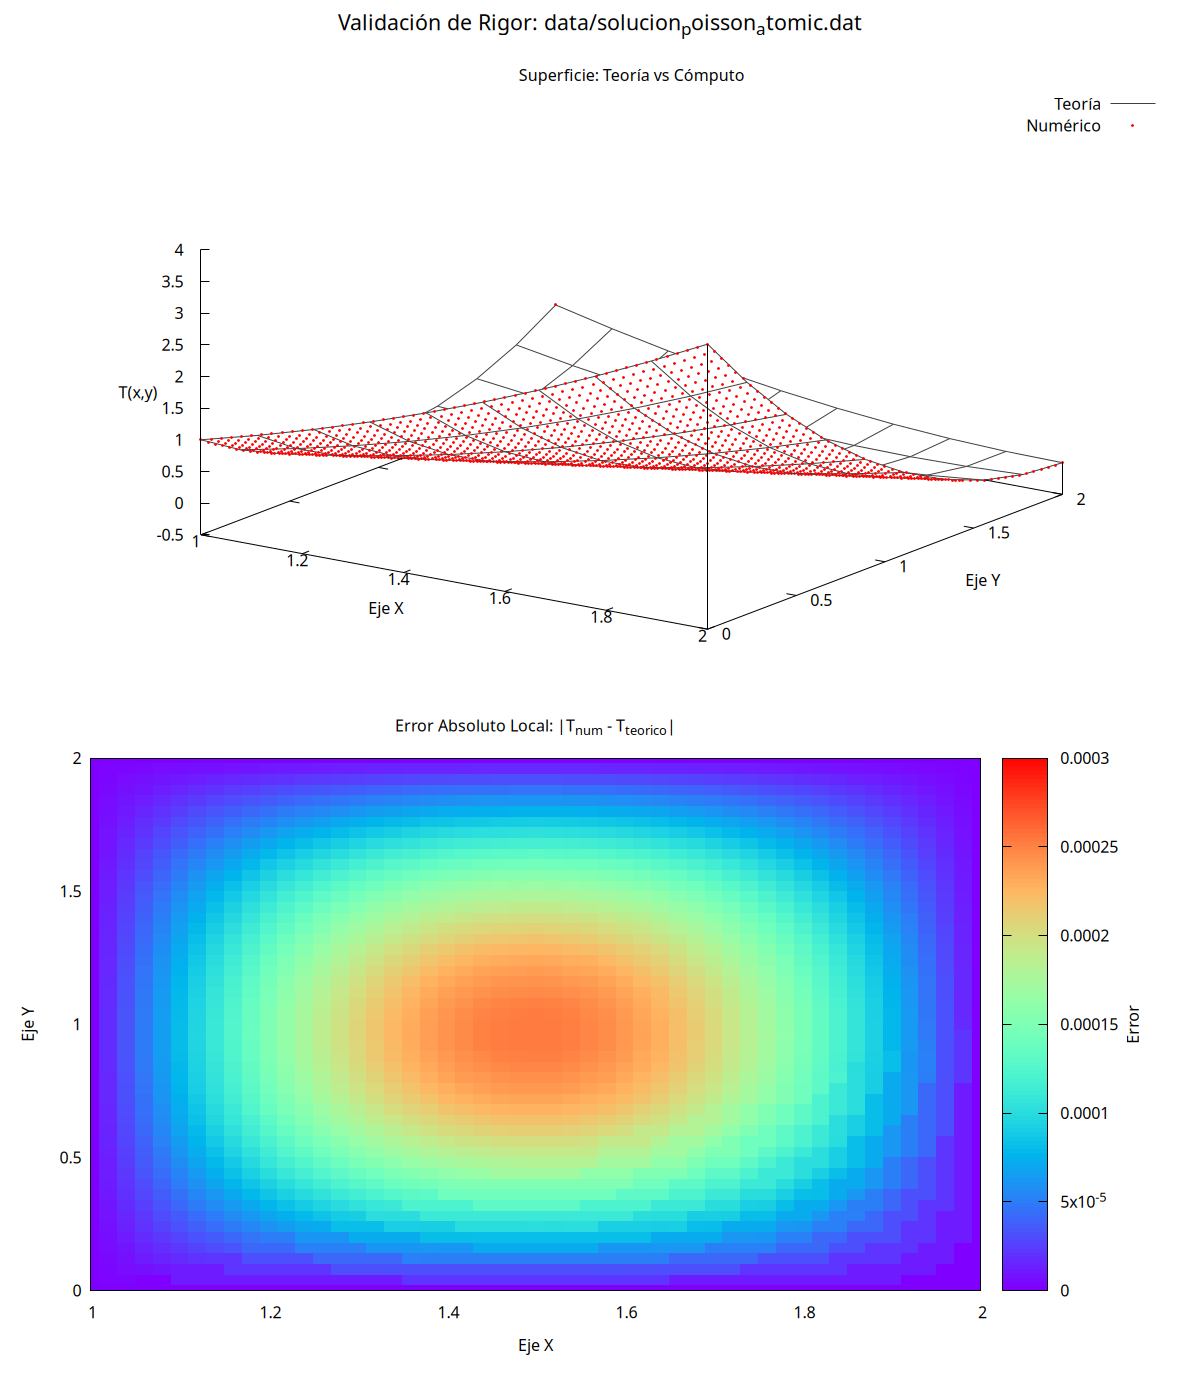
\includegraphics[width=0.65\textwidth]{../../imag/solucion_poisson_atomic.png}
    \caption{Solución numérica de la ecuación de Poisson 2D para una malla $50\times50$ usando la implementación \texttt{atomic}.}
    \label{fig:atomic_sol}
\end{figure}

La solución obtenida reproduce correctamente la forma parabólica esperada, consistente con las condiciones de frontera impuestas y el término fuente constante $f(x,y)=4$. El error numérico global se mantiene acotado por la tolerancia impuesta en el método iterativo, $\text{TOL} = 10^{-6}$, garantizando convergencia del esquema de diferencias finitas.

Para validar la robustez de las implementaciones, se compararon los resultados de todas las versiones paralelas (\texttt{parallel for}, \texttt{collapse}, \texttt{schedule}, \texttt{atomic}, \texttt{critical}, \texttt{sections}, \texttt{task}) sobre la misma malla y bajo las mismas condiciones iniciales.

El análisis estadístico multimodelo, mostrado en la Figura \ref{fig:stats}, permite evaluar la dispersión entre soluciones mediante el cálculo del promedio y bandas de desviación estándar en cada punto de la malla.

\begin{figure}[H]
    \centering
    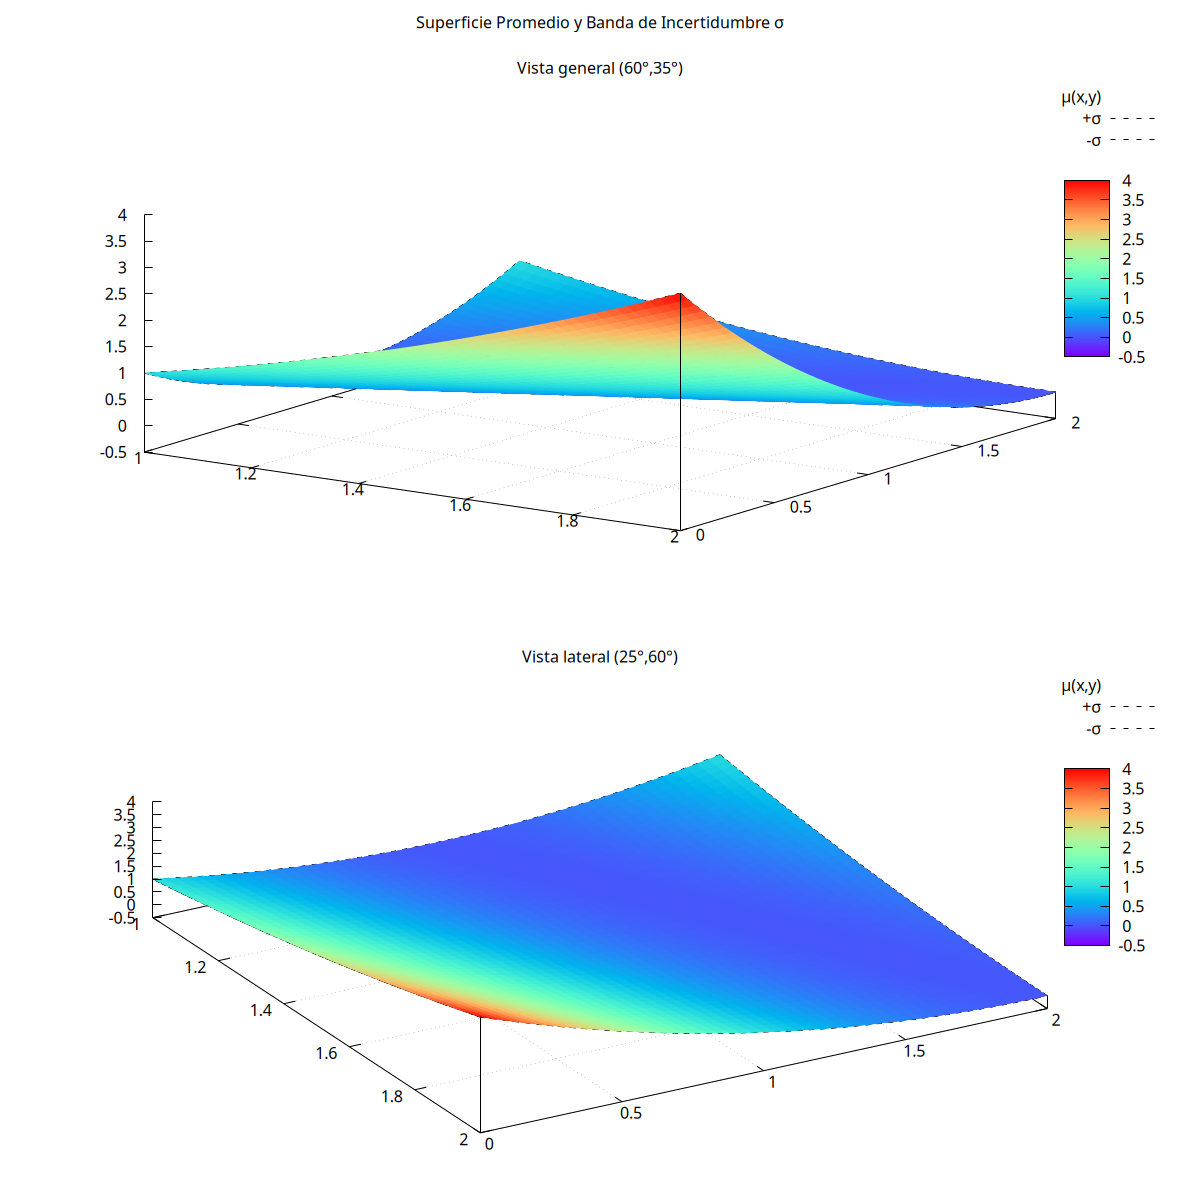
\includegraphics[width=0.75\textwidth]{../../imag/validacion_stats.png}
    \caption{Validación estadística de las soluciones numéricas. Se muestra la superficie promedio junto con bandas de desviación estándar entre implementaciones.}
    \label{fig:stats}
\end{figure}

Los resultados evidencian que todas las implementaciones convergen a la misma solución dentro de la precisión numérica del método, presentando desviaciones despreciables del orden de máquina. Esto confirma que las diferencias observadas en rendimiento no afectan la validez física ni la estabilidad del esquema numérico.

\textbf{Conclusión de validación:} Las variaciones entre implementaciones son exclusivamente computacionales (tiempo de ejecución y escalabilidad), mientras que la solución numérica permanece invariante, validando correctamente todas las estrategias de paralelización implementadas.

\section*{Conclusiones Generales}
\begin{enumerate}
    \item \textbf{¿Cuál fue la versión más rápida y la más eficiente?} \\
    La directiva \texttt{\#pragma omp parallel for} con una planificación básica. Además, se comprobó que el máximo rendimiento se alcanza a los \textbf{32 hilos}, superando ese umbral el paralelismo se vuelve contraproducente por el costo de comunicación y transferencia a caché.

    \item \textbf{¿Qué directiva es más fácil de usar y robusta?} \\
    Nuevamente \texttt{parallel for} con la cláusula \texttt{reduction}. Proporciona el máximo rendimiento con la menor cantidad de intervención en el código base, manteniendo la estabilidad del esquema numérico.

    \item \textbf{¿Hubo directivas que empeoraron el rendimiento?} \\
    De forma contundente, la directiva \texttt{task}. Para la resolución de ecuaciones diferenciales en grillas matriciales uniformes y densas, el modelo de bucles (\texttt{for}) es superior. Las tareas (\texttt{task}) solo deben usarse para flujos de control asimétricos o estructuras irregulares (árboles, listas recursivas).

    \item \textbf{¿La paralelización afectó la validez numérica del método?} \\
    No. Todas las implementaciones convergen a la misma solución dentro de la tolerancia impuesta ($10^{-6}$), reproduciendo correctamente el comportamiento analítico esperado del problema de Poisson con término fuente constante. Se verificó estabilidad y consistencia del método de diferencias finitas, evidenciando que las variaciones entre versiones son exclusivamente computacionales y no físicas.
\end{enumerate}

\end{document}
